%%%%%%%%%%%%%%%%%%%%%%%%%%%%%%%%%%%%%%%%%%%%%%%%%%
%	PRISON PHONE PAPER 
%%%%%%%%%%%%%%%%%%%%%%%%%%%%%%%%%%%%%%%%%%%%%%%%%%
\documentclass[12pt,a4paper]{article}

%%%%%%%%%%%%%%%%%%%%%%%%%%%%%%%%%%%%%%%%%%%%%%%%%%
%	LOADING PACKAGES 
%%%%%%%%%%%%%%%%%%%%%%%%%%%%%%%%%%%%%%%%%%%%%%%%%%
\usepackage{geometry}
\usepackage{graphicx}
\usepackage{tikz}
\usepackage{hyperref}
\usepackage{epstopdf}
\usepackage{amsmath}
\usepackage{pdfpages}
\usepackage{indentfirst}
\usepackage{xurl}
\usepackage{float}
\usepackage{multirow}
\usepackage{booktabs}
\usepackage{caption}
\usepackage{setspace}

%%%%%%%%%%%%%%%%%%%%%%%%%%%%%%%%%%%%%%%%%%%%%%%%%%
%	CUSTOM COMMANDS, ETC. 
%%%%%%%%%%%%%%%%%%%%%%%%%%%%%%%%%%%%%%%%%%%%%%%%%%
\hypersetup{breaklinks=true}
%\newcommand{\sym}[1]{\rlap{$#1$}} % for symbols in Table
\newcommand{\sym}[1]{{#1}} % for symbols in Table

%%%%%%%%%%%%%%%%%%%%%%%%%%%%%%%%%%%%%%%%%%%%%%%%%%
%	TITLE PAGE 
%%%%%%%%%%%%%%%%%%%%%%%%%%%%%%%%%%%%%%%%%%%%%%%%%%
\begin{document}
\title{Communication Costs and Prison Safety: Null Effects of FCC Phone Rate Caps on Inmate Sexual Assaults}
\author{David Ford}
\maketitle
\footnote{DRAFT - DO NOT CIRCULATE} \\

%%%%%%%%%%%%%%%%%%%%%%%%%%%%%%%%%%%%%%%%%%%%%%%%%%
%	ABSTRACT 
%%%%%%%%%%%%%%%%%%%%%%%%%%%%%%%%%%%%%%%%%%%%%%%%%%
\section{Abstract}
This paper examines the impact of reduced communication costs on inmate well-being and safety in U.S. correctional facilities. Leveraging the 2014 Federal Communication Commission (FCC) mandate that imposed caps on prison phone rates, I assess whether lifting financial barriers to communication affects reported sexual assault rates. The analysis combines manually-collected data from prison telecommunications contracts with administrative records on inmate sexual assault reports. Using difference-in-differences and event study designs, I estimate the causal effects of the rate cap on inmate safety outcomes. Across specifications, I find no statistically significant effects of reduced phone costs on reported assaults. These null results suggest that while easing financial constraints on communication may enhance inmate welfare along other dimensions, phone rate reforms alone do not appear to meaningfully influence safety or reporting outcomes within correctional facilities. \\

%%%%%%%%%%%%%%%%%%%%%%%%%%%%%%%%%%%%%%%%%%%%%%%%%%
%	DISSERTATION CHAPTER CONVERSION STEPS 
%%%%%%%%%%%%%%%%%%%%%%%%%%%%%%%%%%%%%%%%%%%%%%%%%%
%	Remove everything above here
%	Remove \end{document}
%	Remove appendix, bibliography
%\chapter[Chapter 2]{Communication Costs and Prison Safety: Null Effects of FCC Phone Rate Caps on Inmate Sexual Assaults}
%\addcontentsline{lof}{chapter}{\numberline{\thechapter}Chapter 2}
%\addcontentsline{lot}{chapter}{\numberline{\thechapter}Chapter 2}
%	overwrite ``chapter2'' file 

\graphicspath{{C:/Users/david/coding/01_PRISON_PHONE_paper/6000_LaTeX/}}

%%%%%%%%%%%%%%%%%%%%%%%%%%%%%%%%%%%%%%%%%%%%%%%%%%
%	INTRODUCTION 
%%%%%%%%%%%%%%%%%%%%%%%%%%%%%%%%%%%%%%%%%%%%%%%%%%
\section{Introduction}
With few alternatives, inmates rely heavily on phone calls to communicate with their friends and family. Additionally, many inmates have no access to jobs, and those that do have access are oftentimes paid wages below the standard federal minimum wage. With direct costs upwards of \$15 for a 15-minute phone call in numerous states, phone calls may be difficult to afford for many state prisoners. \\

When it comes to prisons, policymakers have concerns regarding violence and assaults between inmates, or between inmates and staff. I use a difference in differences estimation combined with event studies to explore the relationship between increased ability to communicate with the outside world via more affordable phone rates, and reports of sexual assault as measured by the Prison Rape Elimination Act (PREA) of 2003. In this estimation, the treatment group are those states which are constrained by the early-2014 FCC phone rate caps, and the control group are those states which were already below the caps in 2013. The study focuses on the years 2008-2018, as data before and after this range is unavailable. Excluding Hawaii, I consider 49 states, with 26 states in the treatment group and 23 states in the control group. \\ 

In September 2003, the United States enacted the PREA in order to better track and reduce the incidence of sexual assault perpetrated on inmates. As a result of this act, state prisons were required to monitor various forms of sexual assault and uniformly report their findings to a federal governing body. \\

Using this PREA data, as well as phone rate data collected by Prison Phone Justice and supplemented by my own searches through contracts between state Departments of Correction and phone companies, I investigate whether those states constrained by the FCC phone caps saw a significant change in reported sexual assaults following the FCC phone rate caps. \\

As evidence to support the relevancy between prison phone call costs and call volume, I have found San Francisco and New York City articles (sfgov.org and nypost.com respectively) that support my prior assumptions. In August 2020, SF made jail phone calls free and reportedly saw a 41\% call volume increase ``overnight''. Further, SF jails reported a 30\% increase in 2016 when they reduced the price of a call from \$2.75 to \$2.10. In August 2018, NYC similarly made jail phone calls free and afterwards saw a 30\% increase in call volumes. \\

%%%%%%%%%%%%%%%%%%%%%%%%%%%%%%%%%%%%%%%%%%%%%%%%%%
%	LITERATURE REVIEW 
%%%%%%%%%%%%%%%%%%%%%%%%%%%%%%%%%%%%%%%%%%%%%%%%%%
\section{Literature Review}
In the previous literature, it has been shown that overcrowding and prison assault volumes are linked in California, a state which has particularly-robust public prison data (Kurtzville, 2017). \\

Additionally, suicide is twice as common among U.S. inmates than the general population, and the third leading cause of prison death after natural causes and AIDS, measures which may even be under-reported with some suicides being rules as accidental deaths (Suto \& Arnaut, 2010). \\

Other studies have shown that inmates who report near-lethal self harm and suicide attempts also report significantly lower social support levels (Sanchez et al, 2021). Studies also find that inmates reporting suicide attempts in prison also report none or few close friends outside of prison, as well as less phone calls and visits from family and friends during their imprisonment (Rivlin et al, 2013). Both of which demonstrate prominently that social support can increase inmate feelings of belonging, and reduce suicide risks. \\

As for the prison telecom industry, inmate telephone businesses comprise a \$1.2B industry, with nearly 90\% of prisoners of state prisons using services provided by just three companies. Despite this large funding and oligopolistic structure, inmates claim that 40\% of prison phone calls fail to connect, which may shift the financial burden onto those families whose calls do connect (Slackman, 2014). \\

Finally, with prison wages typically sub-\$/hour, the phone call cost burden tends to fall on the families and friends of inmates, who tend to be low-income relative to the general U.S. population. Ability to maintain family and community connections act as powerful predictors of re-offending rates post-incarceration, and the FCC themselves point out that implementing rate caps increased inmate call volumes without compromising correctional facility security requirements (Fuchs, 2019). 

%%%%%%%%%%%%%%%%%%%%%%%%%%%%%%%%%%%%%%%%%%%%%%%%%%
%	DATA DESCRIPTION 
%%%%%%%%%%%%%%%%%%%%%%%%%%%%%%%%%%%%%%%%%%%%%%%%%%
\section{Data Description}
\subsection{Prison Rape Elimination Act (PREA) Data} 
Established in 2003, there are a number of metrics that are tracked by state-year through 2018. The number of prisoners in custody on December 31st; inmate non-consensual acts, both alleged and substantiated; inmate abusive contact, both alleged and substantiated; staff sexual misconduct, both alleged and substantiated; and staff sexual harassment, both alleged and substantiated. \\

By appending each available PREA data set, I construct panel data tracking these sexual assault outcome reporting volumes across time to be used as outcome variables to measure inmate well-being surrounding phone rate decreases. Due to much larger allegation volumes relative to substantiations, I elect to focus on the allegation version of each outcome, and stemming from those same reporting volume concerns, I also focus on inmate non-consensual act and staff misconduct reports, both of which have relatively high frequencies in the data. \\

\begin{center}
	\begin{table}[!h]
\caption{Raw Differences}
\centering
\begin{tabular}{llll}
\cline{1-4}
\multicolumn{1}{r}{} &
  \multicolumn{3}{c}{Treatment Status} \\
\multicolumn{1}{r}{} &
  \multicolumn{1}{c}{Control} &
  \multicolumn{1}{c}{Treated} &
  \multicolumn{1}{c}{Total} \\
\cline{1-4}
\multicolumn{1}{l}{Inmate Sexual Acts} &
  \multicolumn{1}{r}{50.72 (77.67)} &
  \multicolumn{1}{r}{49.59 (73.45)} &
  \multicolumn{1}{r}{50.05 (75.13)} \\
\multicolumn{1}{l}{Staff Misconduct} &
  \multicolumn{1}{r}{79.56 (118.28)} &
  \multicolumn{1}{r}{67.79 (132.30)} &
  \multicolumn{1}{r}{72.60 (126.79)} \\
\multicolumn{1}{l}{Pre-Period Cost (\$)} &
  \multicolumn{1}{r}{2.26 (1.01)} &
  \multicolumn{1}{r}{9.70 (4.10)} &
  \multicolumn{1}{r}{6.66 (4.88)} \\
\multicolumn{1}{l}{Prison Pop.} &
  \multicolumn{1}{r}{22594 (21870)} &
  \multicolumn{1}{r}{24996 (34296)} &
  \multicolumn{1}{r}{24016 (29855)} \\
\cline{1-4}
\end{tabular}
\end{table}

\end{center}

\subsection{Prison Phone Justice: Telecom Contracts \& Rates} 
To construct my continuous treatment variable, I manually-pull prison phone rates from a large set of telecommunications contracts, publicly-available information which has been compiled by the Prison Phone Justice initiative, available at \url{prisonphonejustice.org}. By scouring these contracts, I construct a more comprehensive phone rate data set than previously available, allowing me to determine which states had phone rates above the FCC \$0.25/minute (\$3.75/15m) rate caps implemented in 2014. \\

\begin{figure}
	\begin{center}
		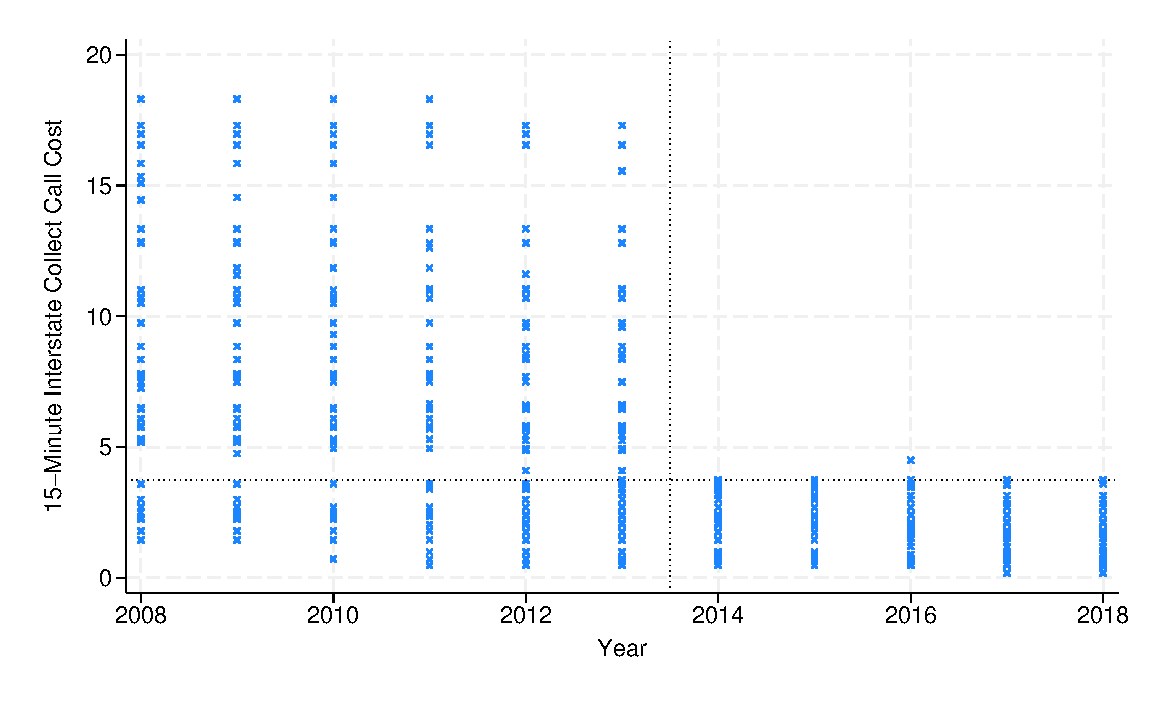
\includegraphics[width=4.5in]{rates_scatterplot.eps}
		\caption[15-Minute Phone Rate Scatterplot]{This figure depicts 15-minute interstate collect call costs before and after the 2014 FCC rate cap went into effect. The states which lie above \$3.75 constitute my treated departments.}
		\label{rate_drop_graph}
	\end{center}
\end{figure}

%%%%%%%%%%%%%%%%%%%%%%%%%%%%%%%%%%%%%%%%%%%%%%%%%%
%	METHODOLOGY & RESULTS 
%%%%%%%%%%%%%%%%%%%%%%%%%%%%%%%%%%%%%%%%%%%%%%%%%%
\section{Methodology and Results}
In order to assess inmate changes in well-being following the aforementioned phone rate decreases, which have been shown to be quite substantial in many cases, I utilize difference-in-differences equations coupled with an event study design. Those states which were above the FCC cap prior to its enactment will be considered treated, and those states which were already adhering to the cap before its enactment will be considered control. Due to timing concerns surrounding the announcement vs enactment of the policy, I also consider states which show large rate decreases in the interim period as treated groups, as they may have preempted the policy during their ongoing contract negotiations to avoid needed to re-negotiate in the near future. \\

To this end, I run the following regressions, discussed below. 

\begin{equation}
	Y^{o}_{s,y} = \alpha + \beta RateDrop_{s,y} + \boldsymbol{X'}_{s,y} \boldsymbol{\gamma} + \boldsymbol{\theta}_{s} + \boldsymbol{\eta}_{y} + u_{s,y}
	\label{eq1_DiD_TWFE}
\end{equation}

Equation \ref{eq1_DiD_TWFE}, a difference-in-differences equation with continuous treatment is used in specifications (1) and (2). $Y^{o}_{s,y}$ refer to my outcomes of interest; Alleged Inmate Non-Consensual Sexual Acts and Alleged Staff Sexual Misconduct. $RateDrop$ denotes the magnitude of the phone rate decrease for treated groups in the post-period. $\boldsymbol{X'}$ denotes my control variables, consisting of total prison population in (1) and adding population-squared in (2). I further utilize both state and year fixed effects, $\theta_{s}$ and $\eta_{y}$ respectively, in order to control for unit- and time-invariant unobserved characteristics which may otherwise bias results. Errors are clustered at the state level. 

\begin{equation}
	Y^{o}_{s,y} = \alpha + \beta RateDrop_{s,y} + \boldsymbol{X'}_{s,y} \boldsymbol{\gamma} + \boldsymbol{\bar{X}}_{s} \boldsymbol{\zeta}_1 + \boldsymbol{\bar{X}}_{y} \boldsymbol{\zeta}_2 + u_{s,y}
	\label{eq2_DiD_TWM}
\end{equation}

Following from Wooldridge (2021), I explore treatment effect heterogeneity by utilizing the Two-Way Mundlak device in equation \ref{eq2_DiD_TWM} which is used in specification (3). Here, $\boldsymbol{\bar{X}}_{s}$ denotes the state-average of each independent variable, and $\boldsymbol{\bar{X}}_{y}$ to the year-averages, acting similarly to unit and time fixed effects. 

\begin{equation}
	\begin{split}
		Y^{o}_{s,y} = \alpha + \beta RateDrop_{s,y} + \boldsymbol{X'}_{s,y} \boldsymbol{\gamma} + \boldsymbol{\bar{X}}_{s} \boldsymbol{\zeta}_1 + \boldsymbol{\bar{X}}_{y} \boldsymbol{\zeta}_2 + \boldsymbol{\bar{X}}_{s} \boldsymbol{\bar{X}}_{y} \boldsymbol{\zeta}_3 \\ 
			+ \boldsymbol{X}_{s,y} (\boldsymbol{\bar{X}}_{s} - \bar{X}) \boldsymbol{\zeta}_4 + \boldsymbol{X}_{s,y} (\boldsymbol{\bar{X}}_{y} - \bar{X}) \boldsymbol{\zeta}_5 + u_{s,y}
		\label{eq3_DiD_TWM_int}
	\end{split}
\end{equation}

The TWM device from equation \ref{eq2_DiD_TWM} is further expanded upon in equation \ref{eq3_DiD_TWM_int} to further explore heterogeneous treatment effects. Here, $\boldsymbol{\bar{X}}$ refers to the grand-average of each covariate, and by differencing this from the state- and year-averages, I allow for different outcome pathways for various treated groups. 

\begin{equation}
	\begin{split}
		Y^{o}_{s,y} = \alpha + \sum^{3}_{k=-3} \beta_{k} D^{k}_{s,y} + \boldsymbol{\theta}_{s} + \boldsymbol{\eta}_{y} + u_{s,y}
		\label{eq4_estudy}
	\end{split}
\end{equation}

Finally, event study equation \ref{eq4_estudy} is used to explore pre-treatment trends and post-treatment outcome paths relative to the year in which a state has a large decrease in their prison phone rates, due to concerns with some states appearing to preempt the FCC caps following their announcement ahead of the enactment. $D^{k}$ is a binary variable indicating which year an observation takes place in relative to that state's rate reduction. \\

\begin{figure}
	\begin{center}
		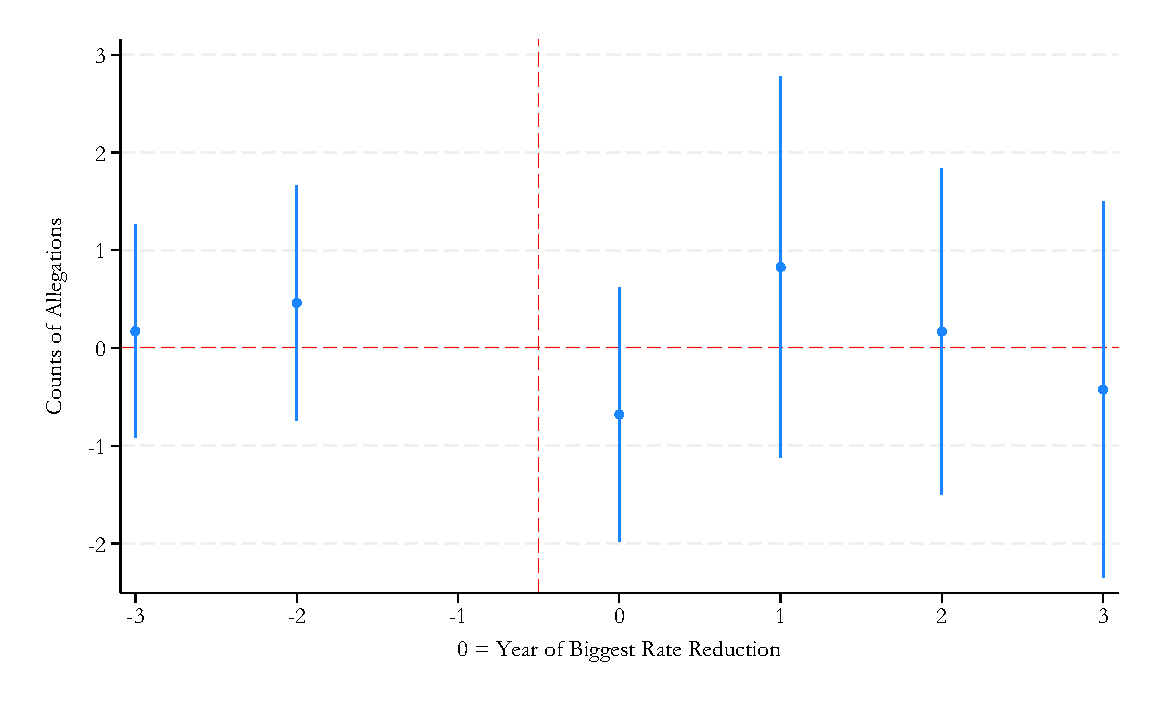
\includegraphics[width=4.5in]{inmate_noncon_all.eps}
		\caption[Alleged Inmate Non-Consensual Sexual Acts Event Study]{This figure depicts event study estimates taken from equation \ref{eq4_estudy}. Following a rate reduction, there does not appear to be a discernible effect on non-consensual sexual act allegations.}
		\label{inmate_noncon_all}
	\end{center}
\end{figure}

\begin{figure}
	\begin{center}
		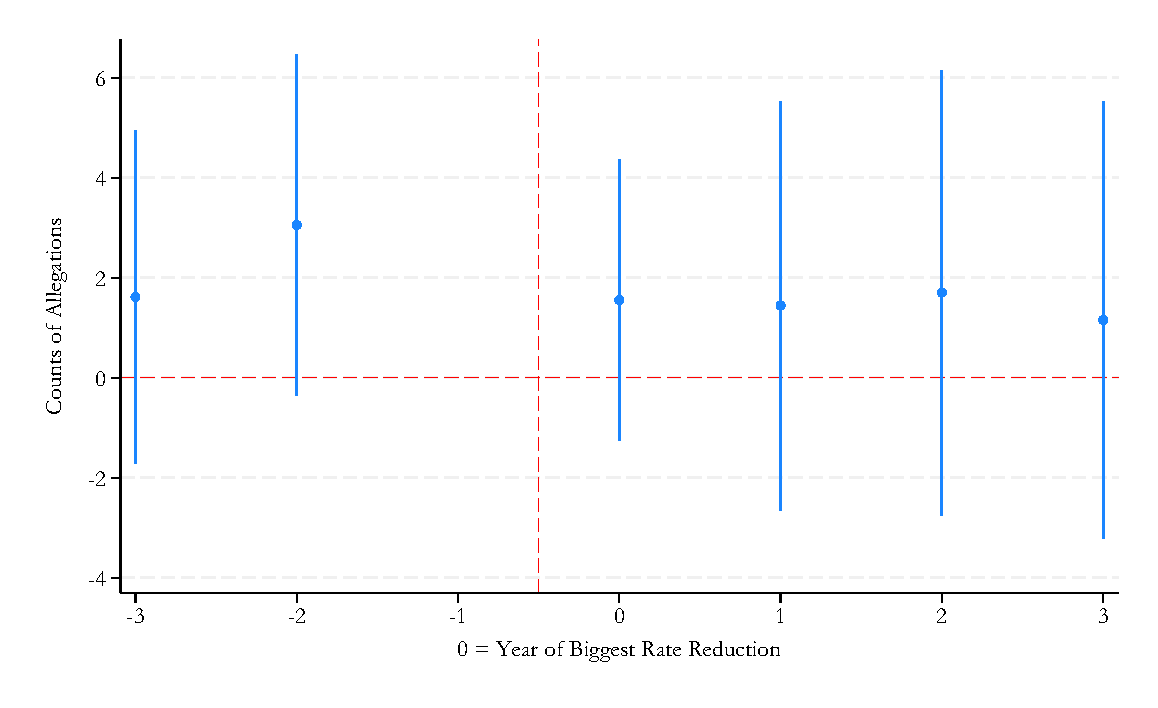
\includegraphics[width=4.5in]{staff_miscond_all.eps}
		\caption[Alleged Staff Sexual Misconduct Event Study]{As in figure \ref{inmate_noncon_all}, there appears to be no treatment effect on staff sexual misconduct allegations.}
		\label{staff_miscond_all}
	\end{center}
\end{figure}

\begin{table}
	\begin{center}
		\input{C:/Users/david/coding/01_PRISON_PHONE_paper/6000_LaTeX/table_inmate_noncon_all_1.1.tex}
		\caption[Inmate Non-Consensual Sexual Act Allegation Estimates]{The models above are derived from equations \ref{eq1_DiD_TWFE}, \ref{eq2_DiD_TWM}, and \ref{eq3_DiD_TWM_int} in columns 1-2, 3 and 4, respectively, which uses a continuous treatment variable $RateDrop_{s,y}$ with state and year fixed effects. Robust standard errors are clustered at the state level. Across various specifications, I find null treatment effect results for the effect of the phone rate drops on Inmate-on-Inmate Non-Consensual Sexual Act Allegations.}
		\label{table_inmate_noncon_all}
	\end{center}
\end{table}

\begin{table}
	\begin{center}
		\begin{tabular}{lcccc} \hline
 & (1) & (2) & (3) & (4) \\
VARIABLES & TWFE & TWFE & TWM & TWM+Int \\ \hline
 &  &  &  &  \\
Treatment & 1.893 & 1.841 & 1.988 & -1.266 \\
 & (2.256) & (2.235) & (2.215) & (2.428) \\
Prison Pop. & -0.006*** & -0.011** & -0.005*** & 0.009*** \\
 & (0.002) & (0.005) & (0.002) & (0.002) \\
Pop. Squared &  & 0.000 &  &  \\
 &  & (0.000) &  &  \\
 &  &  &  &  \\
Observations & 539 & 539 & 517 & 517 \\
 R-squared & 0.616 & 0.618 & 0.403 & 0.556 \\ \hline
\end{tabular}

		\caption[Staff-on-Inmate Sexual Misconduct Allegation Estimates]{This table follows the form of table \ref{table_inmate_noncon_all}, but considers a staff-on-inmate outcome. Across various specifications, I find null treatment effect results for the effect of the phone rate drops on Staff-on-Inmate Sexual Misconduct Allegations.}
		\label{table_staff_miscond_all}
	\end{center}
\end{table}

%%%%%%%%%%%%%%%%%%%%%%%%%%%%%%%%%%%%%%%%%%%%%%%%%%
%	DISCUSSION 
%%%%%%%%%%%%%%%%%%%%%%%%%%%%%%%%%%%%%%%%%%%%%%%%%%
\section{Discussion}
This paper explores whether reduction in financial barriers to communication increase inmate well-being and safety. Across various difference-in-differences specifications, using Two-Way Fixed Effects and Two-Way Mundlak equations and an event study design, I find no statistically significant evidence that phone rate reductions affected sexual assault reporting rates, suggesting that the 2014 FCC rate caps did not meaningfully alter either inmates exposure to, or willingness to report, sexual victimization. \\

Going forward, this question might be further explored using an alternative outcome variable, which may have a more strong and direct potential effect. In particular, the PREA reports are annual data, but the telecommunications contracts for prisons are able to identify which month that a rate reduction went into place, and as such, a monthly outcome variable may be more informative and allow for greater precision. Additionally, there may be some stigma for inmates to report sexual assaults that could be diluting these outcome variables, which may be avoidable using something that is less-able to be censored, such as behavior infractions or prison hospital records. \\

Another avenue for further research could be to consider the subsequent more-restrictive caps implemented by the Biden Administration in 2024, or the 2025 reversal of the caps following an FCC vote. Either of which might give further insights as to the dynamics and effects of financial barriers to inmate communications with their friends and family. \\

Despite this null result, these considerations are important and carry with them important policy applications. Although I do not find any strong effects, it may still be that these financial burdens have an adverse effect on inmate well-being, and these effects are simply too small in magnitude to be measurable in this study. As a captive population with little communication alternatives, it is important to be conscientious of the ability for inmates to feel a sense of belonging and connection with the outside world and to reduce feelings of isolation in correctional settings, in order to both improve their incarceration, as well as their re-integration into society. \\

%%%%%%%%%%%%%%%%%%%%%%%%%%%%%%%%%%%%%%%%%%%%%%%%%%
%	REFERENCES 
%%%%%%%%%%%%%%%%%%%%%%%%%%%%%%%%%%%%%%%%%%%%%%%%%%
\section{References}
Caravaca Sánchez, F., Aizpurua, E., Ricarte, J. J., \& Barry, T. J. (2020). Personal, criminal and social predictors of suicide attempts in prison. Archives of Suicide Research, 25(3), 582–595. \url{https://doi.org/10.1080/13811118.2020.1738293} \\

Fuchs, Z. (2019). Behind Bars: The Urgency and Simplicity of Prison Phone Reform. Harvard Law \& Policy Review, 14(1), 205–229. \\

Kurzfeld, J. (2017). Prison crowding and violent misconduct. SSRN Electronic Journal. \url{https://doi.org/10.2139/ssrn.2994546} \\

Lau, M., \& Stuhldreher, A. (2021, February). Justice is calling how San Francisco made jail phone calls free,. The Financial Justice Project San Francisco. \url{https://www.sfgov.org/financialjustice/files/2021-02/FJP%20Justice%20is%20Calling%202-18-21.pdf} \\

Marsh, J., \& Feis, A. (2019, December 25). Exclusive: NYC inmates made 30 percent more phone calls after they were made free. New York Post. \url{https://nypost.com/2019/12/25/nyc-inmates-made-30-percent-more-phone-calls-after-they-were-made-free/} \\

Rivlin, A., Hawton, K., Marzano, L., \& Fazel, S. (2013). Psychosocial characteristics and social networks of suicidal prisoners: Towards a model of suicidal behaviour in detention. PLoS ONE, 8(7). \url{https://doi.org/10.1371/journal.pone.0068944} \\

Suto, I., \& Arnaut, G. L. (2010). Suicide in prison: A qualitative study. The Prison Journal, 90(3), 288–312. \url{https://doi.org/10.1177/0032885510373499} \\

Wooldridge, J. M. (2021). Two-way fixed effects, the two-way mundlak regression, and difference-in-differences estimators. SSRN Electronic Journal. \url{https://doi.org/10.2139/ssrn.3906345} \\

%%%%%%%%%%%%%%%%%%%%%%%%%%%%%%%%%%%%%%%%%%%%%%%%%%
%	APPENDIX 
%%%%%%%%%%%%%%%%%%%%%%%%%%%%%%%%%%%%%%%%%%%%%%%%%%
\clearpage
\section{Robustness Check: Balanced Panel}
I explore the robustness of my null results by considering a balanced panel, finding similar null results. 

\begin{figure}[H]
	\begin{center}
		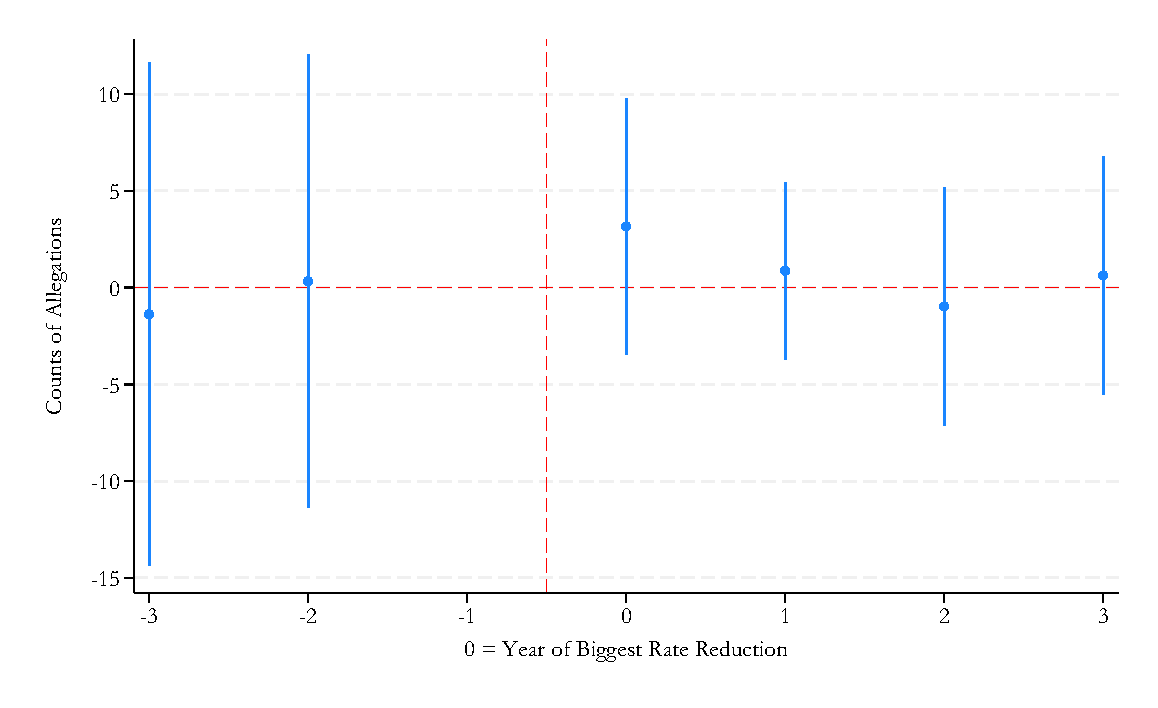
\includegraphics[width=4.5in]{inmate_noncon_all_balanced.eps}
		\caption[Alleged Inmate Non-Consensual Sexual Acts Event Study, Balanced]{As in figure \ref{inmate_noncon_all}, there does not appear to be any significant treatment effect for Inmate-on-Inmate Non-Consensual Sexual Act Allegations.}
		\label{inmate_noncon_all_balanced}
	\end{center}
\end{figure}

\begin{figure}[H]
	\begin{center}
		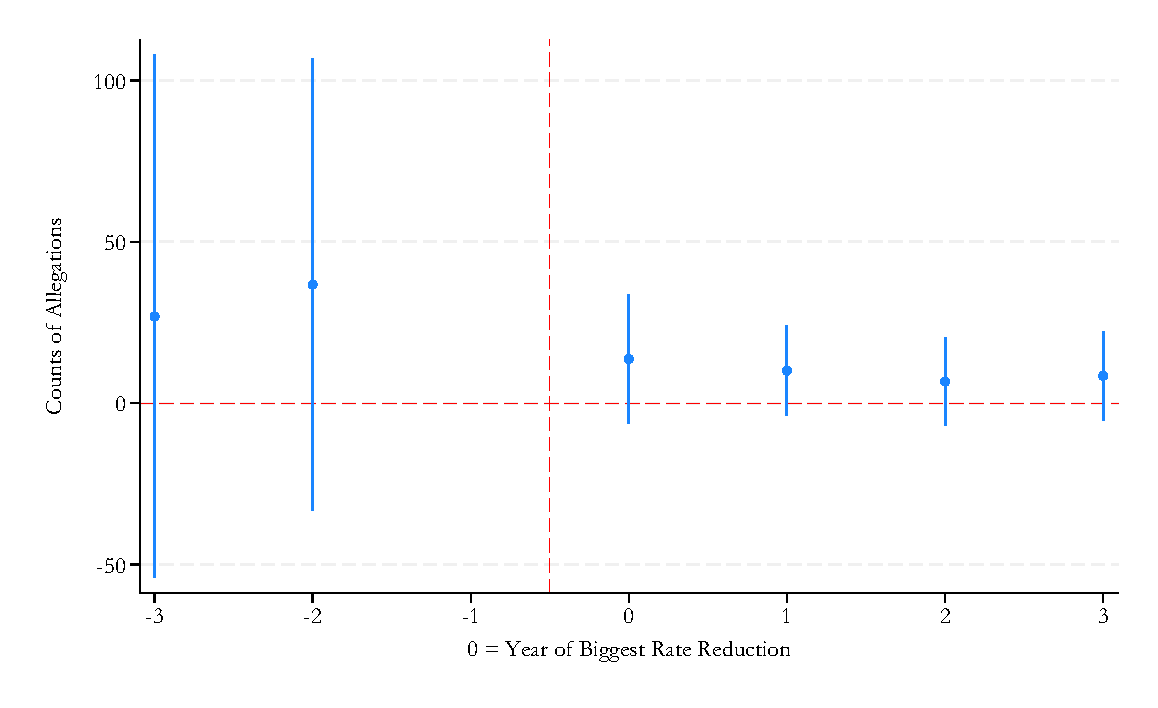
\includegraphics[width=4.5in]{staff_miscond_all_balanced.eps}
		\caption[Alleged Staff Sexual Misconduct Event Study, Balanced]{As in figure \ref{staff_miscond_all}, there does not appear to be any significant treatment effect for Staff-on-Inmate Sexual Misconduct Allegations.}
		\label{staff_miscond_all_balanced}
	\end{center}
\end{figure}

\end{document}
